\chapter{Resolución de artefactos}
En el capítulo anterior hemos visto dos tipos de \textit{funciones de distancia con signo} exactas e inexactas. Las funciones exactas devuelven la escena de manera correcta, ignorando imperfecciones por operaciones de coma flotante. Esto es debido a que la métrica es la euclídea y el \textit{Marcher} siempre traza una esfera con ningún punto en el interior, de ahí su nombre, \textit{Spheremarching}. Cuando tratamos de funciones inexactas, la esferas trazadas también se deforman, por lo que las distancias también lo hacen y por tanto, pueden contener puntos. \\\\
Encontramos dos problemas cuando tratamos de \textit{funciones de distancia con signo inexactas}, en el \textit{Marcher} puede sobreestimar la distancia o subestimar. \\\\

\section{Sobreestimación de la distancia}
Cuando tratamos \textit{funciones de distancia con signo no exactas}, utilizaremos el término \enquote{sobreestimar} cuando se supera la distancia mínima real a la superficie, que es equivalente a que la bola contenga al menos un punto. Encontramos dos formas de  estimar: El rayo trazado se encuentra dentro de la superficie o que el rayo atraviese una superficie. 

\begin{figure}[H]
  \centering
  \subfloat[Se estima dentro de la superficie]{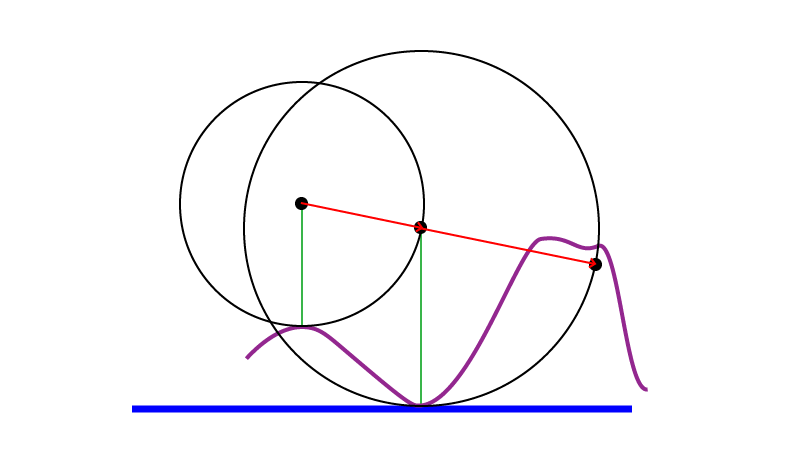
\includegraphics[width=0.45\textwidth]{secciones/imagenes/estimation/sobreestimar-interior.png}}
  \hfill
  \captionsetup{justification=centering}%,margin=2cm
  \subfloat[Se estima fuera de la superficie]{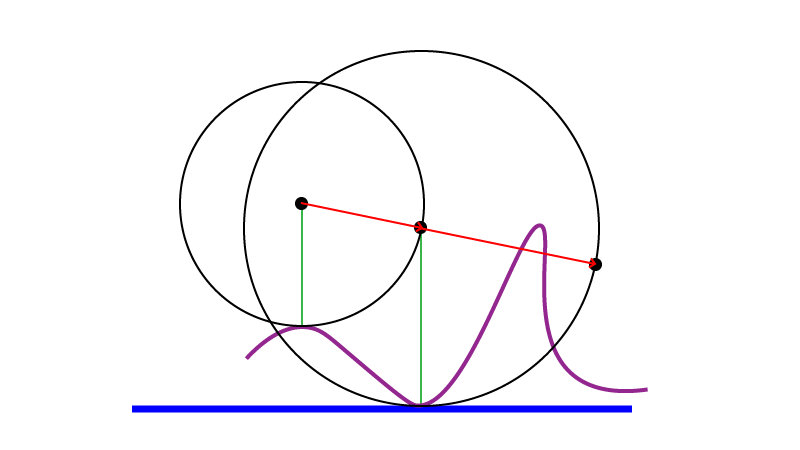
\includegraphics[width=0.45\textwidth]{secciones/imagenes/estimation/sobreestimar-exterior.png}}
  \caption{Dos formas de sobreestimar una superficie}\label{fig:estimacion}
\end{figure}

Es difícil visualizar las circunsferencias deformadas, por lo que se ha realizado un esquema de las dos situaciones que podemos encontrar.

\subsection{Sobreestimación dentro de la superficie}
Tenemos definido estar sobre una superficie cuando \(d_{n+1}<\epsilon\), esta restricción había sido elegida ya que \(d_{n+1}\) siempre es positiva cuando trazamos desde fuera de la superficie. Cuando se sobreestima en el interior de la superficie, la siguiente distancia \(d_{n+1}\) será negativa. Debido a la condición de parada anterior, estos puntos del interior son considerados superficie y el algoritmo terminaría. Para solucionarlo, diremos que estamos sobre una superficie, si y solo si, \( \vert d_{n+1} \vert < \epsilon\), este cambio forzará al \textit{Marcher} a que, en caso de estar en el interior de la superficie, el rayo deba salir de la superficie. Veamos el cambio en el código del algoritmo: 
\begin{lstlisting}
float SphereMarching(
    vec3 ojo, 
    vec3 direccion
){
    float distancia = 0.0;
    for(int i = 0; i < PASOS; ++i){
        vec3 p = ojo + direccion * distancia;
        // d_n+1
        float radio = escena_sdf(p);
        // Estamos sobre la superficie cuando aunque sobreestimemos, no estemos <sobre> la superficie. 
        if(abs(radio) < EPSILON){
            return distancia;
        }
        // Cuando d_n+1 sea negativo, intentará escapar del interior hacia el exterior.
        distancia += radio;
        if(distancia >= MAXIMO) break;
    }
    return MAXIMO;
}
\end{lstlisting}

Veamos el efecto que implica este cambio sobre la deformación vista en \fullref{fig:twist}.

\begin{figure}[H]
  \centering
  \captionsetup{justification=centering}%,margin=2cm
  \subfloat[\textit{Marcher} orginal]{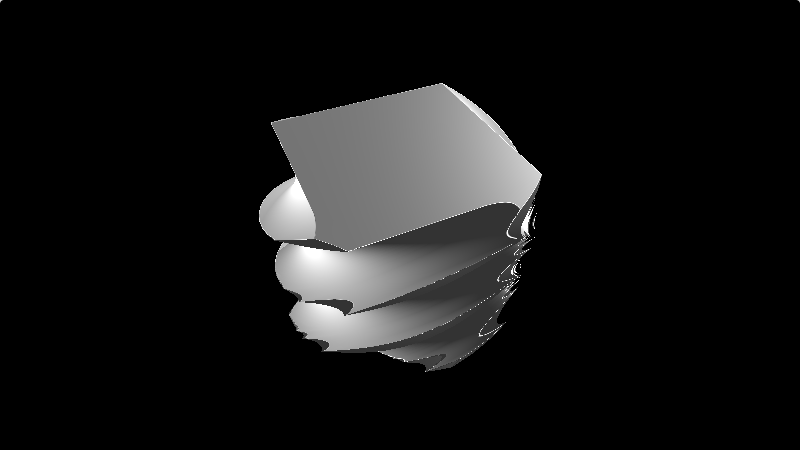
\includegraphics[width=0.45\textwidth]{secciones/imagenes/sdf/3d/sdf_twist.png}}
  \hfill
  \subfloat[\textit{Marcher} sin sobreestimación en el interior]{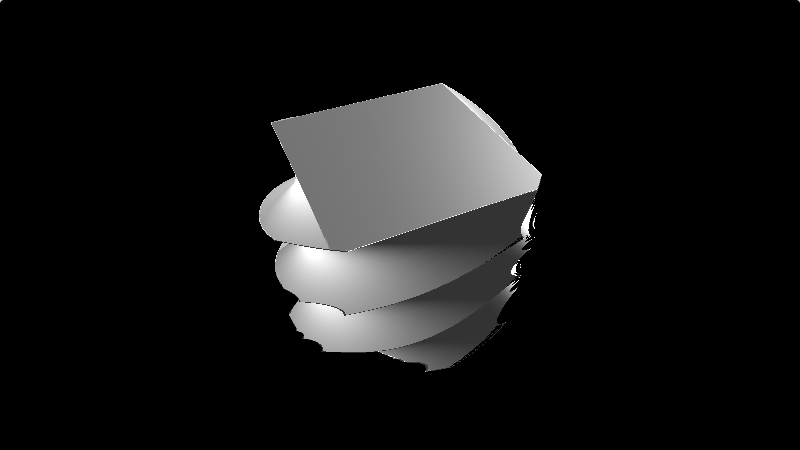
\includegraphics[width=0.45\textwidth]{secciones/imagenes/estimation/sin_sobreestimacion_interior.png}}
  \caption{Comparativa de los cambios realizados en el \textit{Marcher}. A la izquierda, el \textit{Marcher} original, a la derecha, el marcher con \(\vert d_{n+1}\vert < \epsilon\)}
  \label{fig:intestimacion}
\end{figure}

Enlace del ejemplo:\url{https://www.shadertoy.com/view/ttsBDs}

\section{Sobreestimación fuera de la superficie}
Este segundo caso ocurre cuando la deformación aplicada hace que el rayo atraviese la superficie, como ocurre en el ejemplo \textit{(B)}.
Esta sobreestimación afecta considerablemente a la eficiencia del \textit{Marcher}. La solución es escalar en todo momento la bola trazada, obligando a que la bola deformada no pueda contener ningún punto, es decir, sobreestimar. Este cambio nos obligará a utilizar un mayor número de iteraciones, de forma proporcional, para alcanzar la superficie.
\[d'_{n}=d_{n-1} + f(\Vec{p}_{n-1})\cdot k \leq d_{n}\]
Donde \(f\) es nuestra escena; \(k\in[0,1]\) es un factor de escalado de la bola y proporcional al nuevo número de iteraciones. Además, puede ayudar, en ciertas situaciones, a resolver el problema de la \textit{sobreestimación dentro de la superficie}.

\begin{lstlisting}
#define FACTOR_SOBREESTIMACION k
float SphereMarching(
    in vec3 ojo,
    in vec3 direccion, 
    float distancia_plano
){
    float distancia = 0.0;
    for(int i = 0; i < PASOS; ++i){
        vec3 rayo = ojo + direccion * distancia;
        // Escalamos el radio de la esfera
        float radio = escena_sdf(rayo) * FACTOR_SOBREESTIMACION;
        if(abs(radio) < EPSILON){
            return distancia;
        }
        distancia += radio;
        if(distancia > distancia_plano)break;
    }
    return distancia_plano;
}
\end{lstlisting}
Efecto de distintos factores \(k\) al trazado de la escena por el \textit{Marcher}.

\begin{figure}[H]
  \centering
  \captionsetup{justification=centering}%,margin=2cm
  \subfloat[k=1.0]{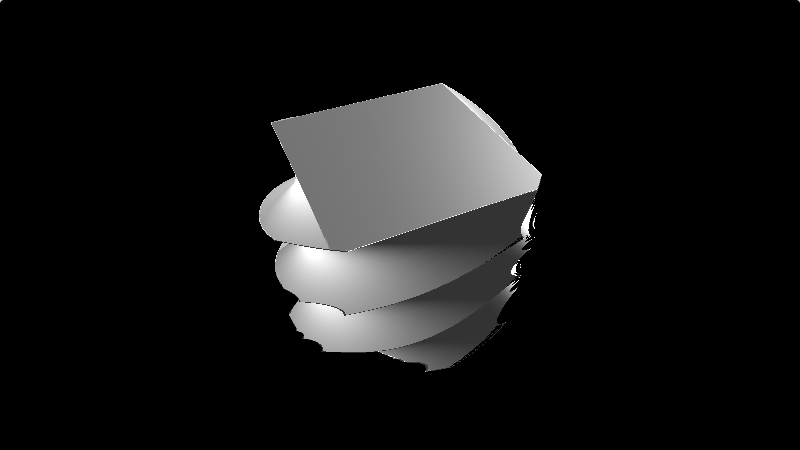
\includegraphics[width=0.3\textwidth]{secciones/imagenes/estimation/sin_sobreestimacion_interior.png}}
  \hfill
  \subfloat[k=0.75]{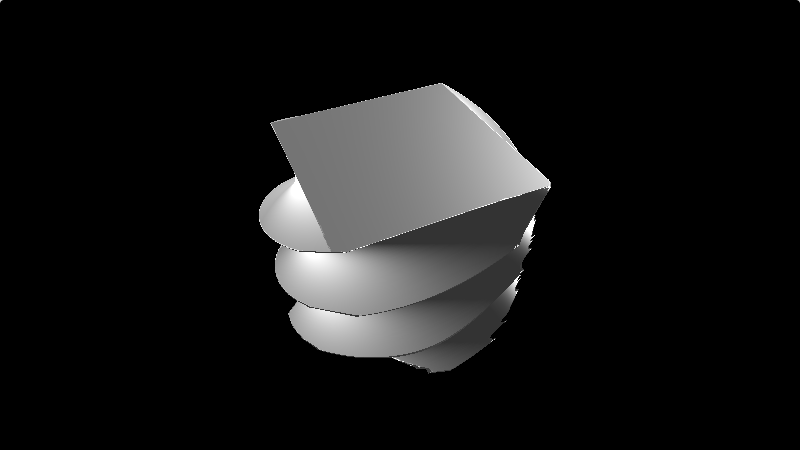
\includegraphics[width=0.3\textwidth]{secciones/imagenes/estimation/sobreestimacion_75.png}}
  \hfill
  \subfloat[k=0.50]{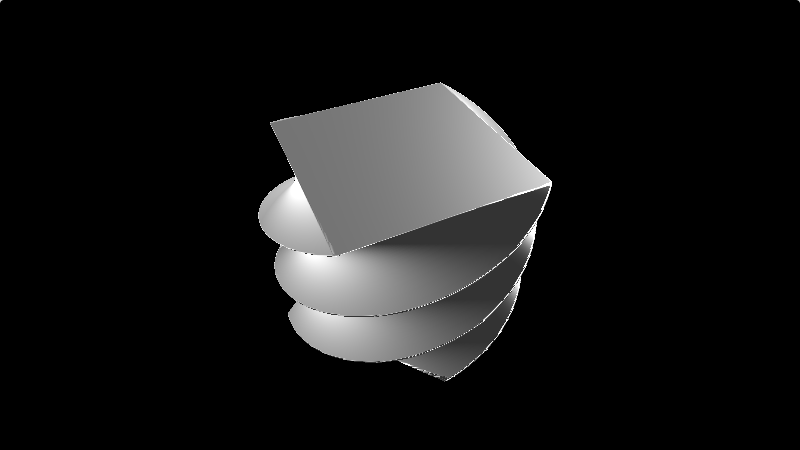
\includegraphics[width=0.3\textwidth]{secciones/imagenes/estimation/sobreestimacion_50.png}}
  \caption{\(k\in\{1, 0.75, 0.5\}\) respectivamente sobre el \textit{Marcher}}
  \label{fig:twistk}
\end{figure}

Enlace del ejemplo:
\url{https://www.shadertoy.com/view/3tBBRR}

%Vemos que la figura es \enquote{exacta} con \(k=0.5\) si observamos la esquina inferior izquierda de la tapadera. Este factor, o reducción de la esfera a la mitad, va a provocar que se requiera el doble de iteraciones para trazar una escena.

\subsection{Subestimación de la distancia}
Este tipo de estimación puede ocurrir tanto en \textit{funciones de distancia con signo exactas como inexactas}. Cuando el \textit{Marcher} finaliza consumiendo todas las iteraciones disponibles, es decir, en la \textbf{Tercera condición}. Por ejemplo, puede ocurrir cuando el rayo pasa de manera paralela, muy cerca a una superficie. Pero, en realidad, no está \enquote{sobre} ella, es decir, \(f(\Vec{rayo}) \ge \epsilon\). La siguiente imagen ilustra este problema:

\begin{figure}[H]
  \centering
  \captionsetup{justification=centering}%,margin=2cm
  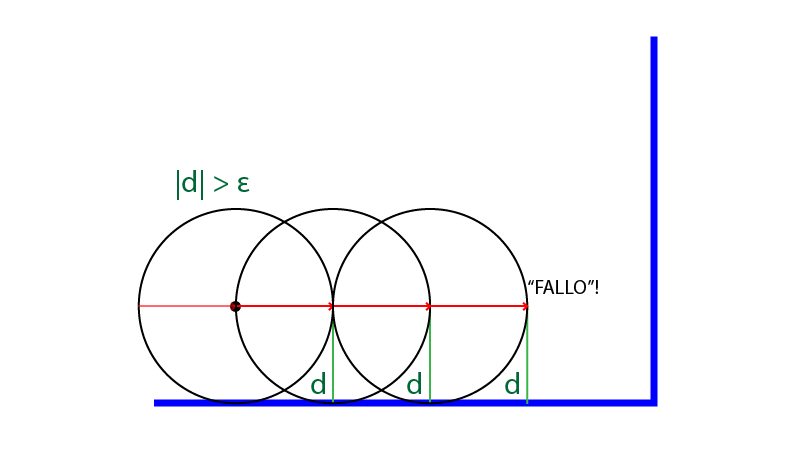
\includegraphics[width=1.0\textwidth]{secciones/imagenes/estimation/subestimacion.png}
  \caption{Ejemplo de subestimación de una superficie}
  \label{fig:subestimacion}
\end{figure}

Estos puntos serán tratados como \enquote{\textit{fallos}} y por tanto, como píxeles de fondo. Utilizar un factor de sobreestimación \(k > 1\) no sería la solución, ya que, crearía \textit{artefactos}. La principal solución es incrementar el número de iteraciones del algoritmo, es decir, incrementar el número de \enquote{\textit{PASOS}}, provocando un mayor gasto computacional. John C. Hart propone en su publicación una optimización para una convergencia rápida en figuras convexas \cite{hart1996sphere} (\enquote{Convexity - Theorem 4}, pág. 534). 